\documentclass{IEEEtran}

\title{IRS-aided SWIPT}
\author{Yang Zhao}
\date{\today}

\usepackage{amsfonts}
\usepackage{amsmath}
\usepackage{amssymb}
\usepackage{cuted}
\usepackage{hyperref}
\usepackage{mathtools}
\usepackage{siunitx}
\usepackage{stfloats}
% \usepackage{nidanfloat}


\begin{document}

% %%%%%%%%%%%%%%%%%%%%%%%%%%%%%%%%%%%%%%%%%
% Academic Title Page
% LaTeX Template
% Version 2.0 (17/7/17)
%
% This template was downloaded from:
% http://www.LaTeXTemplates.com
%
% Original author:
% WikiBooks (LaTeX - Title Creation) with modifications by:
% Vel (vel@latextemplates.com)
%
% License:
% CC BY-NC-SA 3.0 (http://creativecommons.org/licenses/by-nc-sa/3.0/)
%
% Instructions for using this template:
% This title page is capable of being compiled as is. This is not useful for
% including it in another document. To do this, you have two options:
%
% 1) Copy/paste everything between \begin{document} and \end{document}
% starting at \begin{titlepage} and paste this into another LaTeX file where you
% want your title page.
% OR
% 2) Remove everything outside the \begin{titlepage} and \end{titlepage}, rename
% this file and move it to the same directory as the LaTeX file you wish to add it to.
% Then add \input{./<new filename>.tex} to your LaTeX file where you want your
% title page.
%
%%%%%%%%%%%%%%%%%%%%%%%%%%%%%%%%%%%%%%%%%

%----------------------------------------------------------------------------------------
%	PACKAGES AND OTHER DOCUMENT CONFIGURATIONS
%----------------------------------------------------------------------------------------

%----------------------------------------------------------------------------------------
%	TITLE PAGE
%----------------------------------------------------------------------------------------

\begin{titlepage} % Suppresses displaying the page number on the title page and the subsequent page counts as page 1
    \newcommand{\HRule}{\rule{\linewidth}{0.5mm}} % Defines a new command for horizontal lines, change thickness here

    \center % Centre everything on the page

    %------------------------------------------------
    %	Headings
    %------------------------------------------------

    \textsc{\LARGE Imperial College London}\\[1.5cm] % Main heading such as the name of your university/college

    \textsc{\Large Department of Electrical and Electronic Engineering}\\[0.5cm] % Major heading such as course name

    \textsc{\large Communications and Signal Processing Group}\\[4cm] % Minor heading such as course title

    %------------------------------------------------
    %	Title
    %------------------------------------------------


    \HRule \\[0.5cm]
    { \huge \textbf{Waveform and Phase Shift Optimization \\for IRS-aided Wireless Information and Power Transfer}}\\[0.5cm] % Title of your document
    \HRule \\[0.5cm]

    {\large \textit{(Early Stage Report)}}\\[2cm]


    %------------------------------------------------
    %	Author(s)
    %------------------------------------------------

    \begin{minipage}{0.4\textwidth}
        \begin{flushleft}
            \large
            \textit{Author}\\
            Yang \textsc{Zhao} % Your name
        \end{flushleft}
    \end{minipage}
    ~
    \begin{minipage}{0.4\textwidth}
        \begin{flushright}
            \large
            \textit{Supervisor}\\
            Prof. Bruno \textsc{Clerckx} % Supervisor's name
        \end{flushright}
    \end{minipage}

    % If you don't want a supervisor, uncomment the two lines below and comment the code above
    %{\large\textit{Author}}\\
    %John \textsc{Smith} % Your name

    %------------------------------------------------
    %	Date
    %------------------------------------------------

    \vfill\vfill\vfill % Position the date 3/4 down the remaining page

    {\large\today} % Date, change the \today to a set date if you want to be precise

    %------------------------------------------------
    %	Logo
    %------------------------------------------------

    %\vfill\vfill
    %\includegraphics[width=0.2\textwidth]{placeholder.jpg}\\[1cm] % Include a department/university logo - this will require the graphicx package

    %----------------------------------------------------------------------------------------

    \vfill % Push the date up 1/4 of the remaining page

\end{titlepage}

%----------------------------------------------------------------------------------------


\begin{abstract}
	Simultaneous Wireless Information and Power Transfer (SWIPT) is severely restricted by the low power level of the receive Radio-Frequency (RF) signal. To tackle this problem, we introduce Intelligent Reflecting Surface (IRS) that brings a high passive beamforming gain to compensate the propagation loss and boost the energy efficiency with a low power consumption. This paper investigates an IRS-aided Orthogonal Frequency Division Multiplexing (OFDM) SWIPT system based on practical nonlinear harvester model, where a multi-antenna Access Point (AP) transmits information and energy simultaneously to a single-antenna user under the assist of IRS. We aim to maximize the Rate-Energy (R-E) region via jointly optimizing the transmit waveform at the AP, the phase shifts at the IRS, and the splitting ratio at the user. The problem is formulated as current maximization problem subject to rate constraint, and we propose an low-complexity alternating algorithm to obtain suboptimal solutions iteratively. Numerical results demonstrated that dedicated power signal is beneficial to multicarrier SWIPT, while IRS brings significant R-E region enlargement over benchmark schemes when properly configured.
\end{abstract}

\begin{section}{Introduction}
	\begin{subsection}{Simultaneous Wireless Information and Power Transfer}
		With the great advance in communication performance (throughput, latency, outage), the main challenge of wireless network has come to energy supply. Most existing mobile devices are powered by batteries that require frequent charging or replacement, which leads to high maintenance cost and thus restricts the scale of networks. Although solar energy and inductive coupling has become popular alternatives, the former depends on the environment while the latter has a very short operation range. Simultaneous Wireless Information and Power Transfer (SWIPT) is a promising solution to connect and power mobile devices via electromagnetic (EM) waves in the Radio-Frequency (RF) band. It provides low power (in \si{\uW} level) but broad coverage (up to hundreds of meters) \cite{Ng2018} in a sustainable and controllable manner. The decreasing trend in electronic power consumption also boosts the paradigm shift from dedicated power source to Wireless Power Transfer (WPT) and SWIPT.

		The concept of SWIPT were first cast in \cite{Varshney2008}, where the authors investigated the Rate-Energy (R-E) tradeoff for a flat Gaussian channel and some discrete channels. Two practical receiver structures were then proposed in \cite{Zhou2013}, namely Time Switching (TS) that switches between Energy Harvesting (EH) and Information Decoding (ID) modes, and Power Splitting (PS) that splits the received signal into individual components. On top of this, \cite{Zhang2013} characterized the R-E region for a Multiple-Input Multiple-Output (MIMO) broadcast system under TS and PS setup. Information and power beamforming was then considered in multiuser Multi-Input Single-Output (MISO) systems to maximize the Weighted Sum-Power (WSP) subjective to Signal-to-Interference-plus-Noise Ratio (SINR) constraints \cite{Xu2014}. Motivated by this, \cite{Krikidis2014} investigated fundamental transceiver modules, information and power scheduling, and interference management for SWIPT systems. However, \cite{Boshkovska2015} pointed out that the Radio Frequency-to-Direct Current (RF-to-DC) conversion efficiency depends on the harvester input power level, which also suggested a parametric harvester model based on curve fitting and proposed an iterative resource allocation algorithm. From another perspective, \cite{Trotter2009,Boaventura2011} demonstrated that multisine waveform is more suitable for WPT as it outperforms single tone in both operation range and RF-to-DC efficiency. \cite{Clerckx2016a} derived a tractable nonlinear harvester model based on the Taylor expansion of diode I-V characteristics and proposed an adaptive waveform optimization algorithm to maximize the output DC current under rate constraints. Simulation and experiments demonstrated the benefit of modelling rectifier nonlinearity in system design \cite{Kim2019,Kim2019a}. The work was extended to SWIPT in \cite{Clerckx2018} where a superposition of modulated information waveform and multisine power waveform is optimized to enlarge the R-E region. In contrast, \cite{Park2018} suggested an adaptive dual-mode SWIPT, which alternates between single-tone transmission that exploits conventional modulation for high-rate applications and multisine transmission that encodes the information in the Peak-to-Average Ratio (PAPR) for power-demanding applications. By assuming On-Off-Keying (OOK) where bit 1 carries energy, \cite{Hu2019} compared unary and Run-Length-Limited (RLL) code in terms of rate vs battery overflow/underflow probability, and adapted conventional modulation schemes to ensure WPT is only activated at the points with large offset. Also, a learning approach \cite{Varasteh2019c} demonstrated that the offset of the power symbol is positively correlated to the harvester energy constraint, while the information symbols are symmetrically distributed around the origin. It confirmed that the superposed waveform is feasible to enlarge R-E region when considering rectifier nonlinearity. SWIPT was also explored in the network design. \cite{Liu2016} proposed a cooperative SWIPT Non-Orthogonal Multiple Access (NOMA) protocol with three user selection schemes such that the strong user assists the EH of the weak user. In \cite{Mao2019}, SWIPT based on Rate Splitting (RS) was formulated as a Weighted Sum-Rate (WSR) maximization problem subject to total harvested energy constraint for separated Information Receivers (IRs) and Energy Receivers (ERs).
	\end{subsection}

	\begin{subsection}{Intelligent Reflecting Surface}
		Intelligent Reflecting Surface (IRS) adapts the wireless environment to increase spectrum and energy efficiency. In practice, an IRS consists of multiple individual reflecting elements that adjust the amplitude and phase of the incident signal through passive beamforming. Different from relay and backscatter communication, IRS assists the primary transmission without any active components, leading to low power consumption and no thermal noise added to the reflected signal. Compared with the linear increase in Amplify-and-Forward (AF) relay, the received power scales quadratically with the number of reflectors \cite{Wu2019}, since more reflectors boost the power collected by IRS and increase the array gain in its equal gain transmission.

		Inspired by the advance in real-time reconfigurable metamaterials \cite{Cui2014}, \cite{Liaskos2018} introduced a programmable metasurface that steers or polarizes the EM wave at specific frequency to mitigate signal attenuation. At the same time, \cite{Tan2018} constructed an adjustable reflect array that ensures reliable millimeter-wave (mmWave) communication based on a beam-searching algorithm to reduce indoor signal blockage. Motivated by this, \cite{Wu2018,Wu2019} introduced an IRS-assisted MISO system and proposed a beamforming algorithm that jointly optimizes the precoder at the Access Point (AP) and the phase shifts at the IRS to maximize Signal-to-Noise Ratio (SNR). The active and passive beamforming problem was extended to the discrete phase shift case \cite{Wu2019a} and the multiuser case \cite{Guo2019a}. In \cite{Nadeem2019}, channel estimation for Time-Division Duplex (TDD) systems was carried through a two-stage Minimum Mean Squared Error (MMSE)-based protocol that sequentially estimates the cascaded channel of each IRS element with the others switched off. Starting from the impedance equation, \cite{Abeywickrama2019} investigated the influence of phase shift on the reflection amplitude and proposed a parametric IRS model via curve fitting. Recent research also explored the opportunity of integrating IRS with Orthogonal Frequency-Division Multiplexing (OFDM) systems. \cite{Yang2019} exploited spatial correlation to reduce estimation overhead and design complexity by assuming adjacent elements share a common reflection coefficient. On top of this, group-based OFDM channel estimation was investigated in \cite{Zheng2019}. By adjusting IRS over time slots, \cite{Yang2020} introduced artificial diversity within coherence time and investigated resource allocation and IRS configuration per Resource Block (RB). Real-time high-definition video transmission was performed over a prototype constructed with Positive Intrinsic-Negative (PIN) diodes, which demonstrated the feasibility and benefit of IRS at GHz and mmWave frequency \cite{Dai2020}.

		Most existing papers assume a Frequency-Flat (FF) IRS where all elements reflect different frequencies equally. Although Frequency-Selective Surface (FSS) has received much attention for wideband communications, it is prohibitive since active FSS requires RF-chains \cite{Kim2006,Xu2014} while passive FSS has fixed physical characteristics and unable to adjust channel adaptively \cite{Anwar2018}.
	\end{subsection}

	\begin{subsection}{IRS-aided SWIPT}
		The effective channel enhancement and low power consumption of IRS are expected to bring more opportunities to SWIPT. Based on linear harvester model and energy interference, \cite{Wu2019b} proved that at most one energy beam is required to maximize the WSP subject to SINR constraints. The fairness issue was then considered in \cite{Tang2019}, which maximize the minimum output power on the assumption of perfect energy interference cancellation. \cite{Wu2019c} proposed a novel penalty-based algorithm, whose inner layer employs Block Coordinate Descent (BCD) method to update precoders, phase shifts and auxiliary variables while the outer layer updates the penalty coefficients. It demonstrated that Line-of-Sight (LoS) links can boost the harvested power, as the rank-deficient channels are highly correlated and a single energy stream can satisfy the energy constraints of all ERs. In \cite{Pan2019a}, the WSR maximization of MIMO SWIPT was first transformed to Weighted Minimum Mean Square Error (WMMSE) problem then solved by BCD with low-complexity iterative algorithms. However, most existing IRS-SWIPT papers focus on narrow-band transmission over linear harvester model.
	\end{subsection}

	\begin{subsection}{Objective and Methodology}
		In this paper, we study an IRS-aided broadband downlink MISO SWIPT system where the IRS assists the information and energy transmission of a single user. A multicarrier unmodulated power waveform (deterministic multisine) is superposed to a multicarrier modulated information waveform (e.g. OFDM) to boost the energy transfer efficiency without introducing additional interference. The transmit waveform, IRS phase shift and receive splitting ratio are jointly optimized to maximize the R-E tradeoff. Different from previous research, this paper focus on broadband SWIPT and investigates the fundamental impact of harvester nonlinearity on IRS design. We transform the R-E region characterization problem into multiple current maximization problems subject to different rate constraints. To reduce the design complexity, we propose an Alternating Optimization (AO) algorithm that updates the channel and transceiver iteratively based on Semidefinite Relaxation (SDR) and Geometric Programming (GP) technique. Numerical results showed that SDR is tight and the proposed algorithm can find a stationary point for all tested channel realizations. We demonstrate that dedicated power waveform boosts the energy transmission efficiency, such that TS and PS are preferred for low-rate and high-rate applications respectively. Also, IRS brings a significant channel amplification thus R-E enhancement especially when located near the transmitter/receiver, and the performance loss compared with ideal Frequency-Selective (FS) IRS decreases as the number of reflectors increases.
	\end{subsection}
\end{section}

\begin{section}{System Model}
	Consider an IRS-aided SWIPT system where a $M$-antenna transmitter delivers information and power simultaneously, through a $L$-reflector IRS, to a single-antenna user over $N$ orthogonal subbands. We assume a total bandwidth $B$ with evenly-spaced subbands centered at frequency $f_n$ ($n=1,\dots,N$). Perfect Channel State Information (CSI) with negligible training overhead is assumed to explore the analytical upper-bound of the proposed design. A quasi-static block fading channel model is considered for all links, and we focus on one particular block where the channels are approximately unchanged. Two practical co-located receiver architectures are compared in terms of R-E region. Specifically, TS divides each time slot into orthogonal data and energy slots and performs a time sharing between WPT and Wireless Information Transfer (WIT). In comparison, PS splits the received signal into individual ID and EH streams such that the splitting ratio $\rho$ is coupled with waveform and IRS design. Perfect synchronization is assumed among the three parties in both scenarios, and signals reflected by IRS for two and more times are omitted.
	\begin{subsection}{Transmit Signal}
		Denote $\tilde{x}_{I,n}(t)$ as the information symbol transmitted over subband $n$, which follows a capacity-achieving i.i.d. Circular Symmetric Complex Gaussian (CSCG) distribution with zero mean and unit variance $\tilde{x}_{I,n}\sim\mathcal{CN}(0,1)$. The superposed transmit signal on antenna $m$ ($m=1,\dots,M$) at time $t$ is
		\begin{equation}\label{eq:x_m}
			x_m(t)=\Re\left\{\sum_{n=1}^N\left({w_{I,n,m}\tilde{x}_{I,n}(t)}+w_{P,n,m}\right){e^{j2{\pi}{f_n}{t}}}\right\}
		\end{equation}
		where $w_{I/P,n,m}$ denotes the weight on the information and power signal transmitted by antenna $m$ at subband $n$. Define $\boldsymbol{w}_{I/P,n}=[w_{I/P,n,1},\dots,w_{I/P,n,M}]^T \in \mathbb{C}^{M \times 1}$ by stacking up weights across all antennas. Therefore, the transmit information and power signals write as
		% , and let $\boldsymbol{w}_{I/P,n}=\boldsymbol{s}_{I/P,n} e^{j \boldsymbol{\psi}_{I/P,n}}$ such that $\boldsymbol{s}_{I/P,n}$, $\boldsymbol{\psi}_{I/P,n} \in \mathbb{C}^{M \times 1}$ denote the magnitude and phase of the waveform at subband $n$
		\begin{align}
			\boldsymbol{x}_{I}(t) &= \Re{\left\{\sum_{n=1}^N\boldsymbol{w}_{I,n}\tilde{x}_{I,n}(t){e^{j2{\pi}{f_n}{t}}}\right\}}\label{eq:x_I}\\
			\boldsymbol{x}_{P}(t) &= \Re{\left\{\sum_{n=1}^N\boldsymbol{w}_{P,n}{e^{j2{\pi}{f_n}{t}}}\right\}}\label{eq:x_P}
		\end{align}
	\end{subsection}

	\begin{subsection}{Composite Channel}
		At subband $n$, denote the AP-user direct channel as $\boldsymbol{h}_{D,n}^H \in \mathbb{C}^{1 \times M}$, AP-IRS incident channel as $\boldsymbol{H}_{I,n} \in \mathbb{C}^{L \times M}$, and IRS-user reflective channel as $\boldsymbol{h}_{R,n}^H \in \mathbb{C}^{1 \times L}$. At the IRS, element $l$ ($l=1,\dots,L$) redistributes the incoming signal by adjusting the reflection amplitude $\gamma_l \in [0,1]$ and phase shift $\theta_l \in [0,2\pi)$ \footnote{To investigate the performance upper bound of IRS, we suppose the reflection coefficient is maximized $\gamma_l=1 \ \forall l$ while the phase shift is a continuous variable over $[0,2\pi)$.}. On top of this, the IRS matrix collects the reflection coefficients onto the main diagonal entries as $\boldsymbol{\Theta} = \mathrm{diag}(\gamma_1 e^{j \theta_1}, \dots, \gamma_L e^{j \theta_L}) \in \mathbb{C}^{L \times L}$. The extra link introduced by IRS can be modeled as a concatenation of the AP-IRS channel, IRS reflection, and IRS-user channel. On top of this, the total composite channel is formed by adding the IRS-aided extra channel to the AP-user direct channel as
		\begin{equation}\label{eq:h_n}
			\boldsymbol{h}_{n}^H = \boldsymbol{h}_{D,n}^H + \boldsymbol{h}_{R,n}^H \boldsymbol{\Theta} \boldsymbol{H}_{I,n} = \boldsymbol{h}_{D,n}^H + \boldsymbol{\phi}^H \boldsymbol{V}_{n}
		\end{equation}
		where $\boldsymbol{\phi}=[\gamma_1 e^{j \theta_1}, \dots, \gamma_L e^{j \theta_L}]^H \in \mathbb{C}^{L \times 1}$ and $\boldsymbol{V}_{n}=\mathrm{diag}(\boldsymbol{h}_{R,n}^H)\boldsymbol{H}_{I,n} \in \mathbb{C}^{L \times M}$. Note that the Hermitian transpose in the definition of $\boldsymbol{\phi}$ makes its entries complex conjugate of the diagonal entries of $\boldsymbol{\Theta}$.% Let $\boldsymbol{h}_n=\boldsymbol{a}_n e^{j \boldsymbol{\varsigma}_n}$ such that $\boldsymbol{a}_n$, $\boldsymbol{\varsigma}_n \in \mathbb{C}^{M \times 1}$ denote the magnitude and phase of the composite channel at subband $n$.
	\end{subsection}

	\begin{subsection}{Receive Signal}
		At the single-antenna receiver, the total received signal $y(t)=y_I(t)+y_P(t)$ captures the contribution of information and power components over $N$ subbands, where
		\begin{align}\label{eq:y_IP}
			y_{I}(t) & = \Re\left\{\sum_{n=1}^N{\boldsymbol{h}_{n}^H}{\boldsymbol{w}_{I,n}\tilde{x}_{I,n}(t)}{e^{j2{\pi}{f_n}{t}}}\right\}\\
			y_{P}(t) & = \Re\left\{\sum_{n=1}^N{\boldsymbol{h}_{n}^H}\boldsymbol{w}_{P,n}{e^{j2{\pi}{f_n}{t}}}\right\}
		\end{align}
	\end{subsection}

	\begin{subsection}{Information Decoder}
		A major benefit of the proposed waveform is that the determined power waveform creates no interference to the information waveform. Therefore, the achievable rate writes as
		\begin{equation}\label{eq:R}
			\begin{split}
				R(\boldsymbol{\phi},\boldsymbol{w}_I,\rho)
				& = \sum_{n=1}^N{\log_2\left(1+\frac{(1-\rho)\lvert \boldsymbol{h}_{n}^H\boldsymbol{w}_{I,n} \rvert^2}{\sigma_n^2}\right)}\\
				& = \sum_{n=1}^N{\log_2\left(1+\frac{(1-\rho)\lvert(\boldsymbol{h}_{D,n}^H+\boldsymbol{\phi}^H\boldsymbol{V}_n)\boldsymbol{w}_{I,n}\rvert^2}{\sigma_n^2}\right)}
			\end{split}
		\end{equation}
		where $\sigma_n^2$ is the variance of the total noise (RF-band and RF-to-baseband conversion) on tone $n$. Rate \ref{eq:R} is achievable with either waveform cancellation or translated demodulation \cite{Clerckx2018b}.
	\end{subsection}

	\begin{subsection}{Energy Harvester}
		In this section, we briefly revisit a tractable nonlinear rectenna model that relates the harvester output DC current to the received waveform \cite{Clerckx2016a,Clerckx2018b}. Fig. \ref{fi:antenna_equivalent_circuit} illustrates the equivalent circuit of a lossless antenna, where the incoming signal creates an voltage source $v_s(t)$ and the antenna has an impedance $R_{\text{ant}}$. Let $R_{\text{in}}$ be the total input impedance of the rectifier and matching network. Assume the voltage across matching network is negligible and the RF-band noise is too small to harvest. When perfectly matched ($R_{\text{in}}=R_{\text{ant}}$) with power splitting ratio $\rho$, the rectifier input voltage is $v_{\text{in}}(t)=y(t)\sqrt{\rho R_{\text{ant}}}$.

		\begin{figure}
			\centering
			\begin{subfigure}[t]{0.45\linewidth}
				\centering
				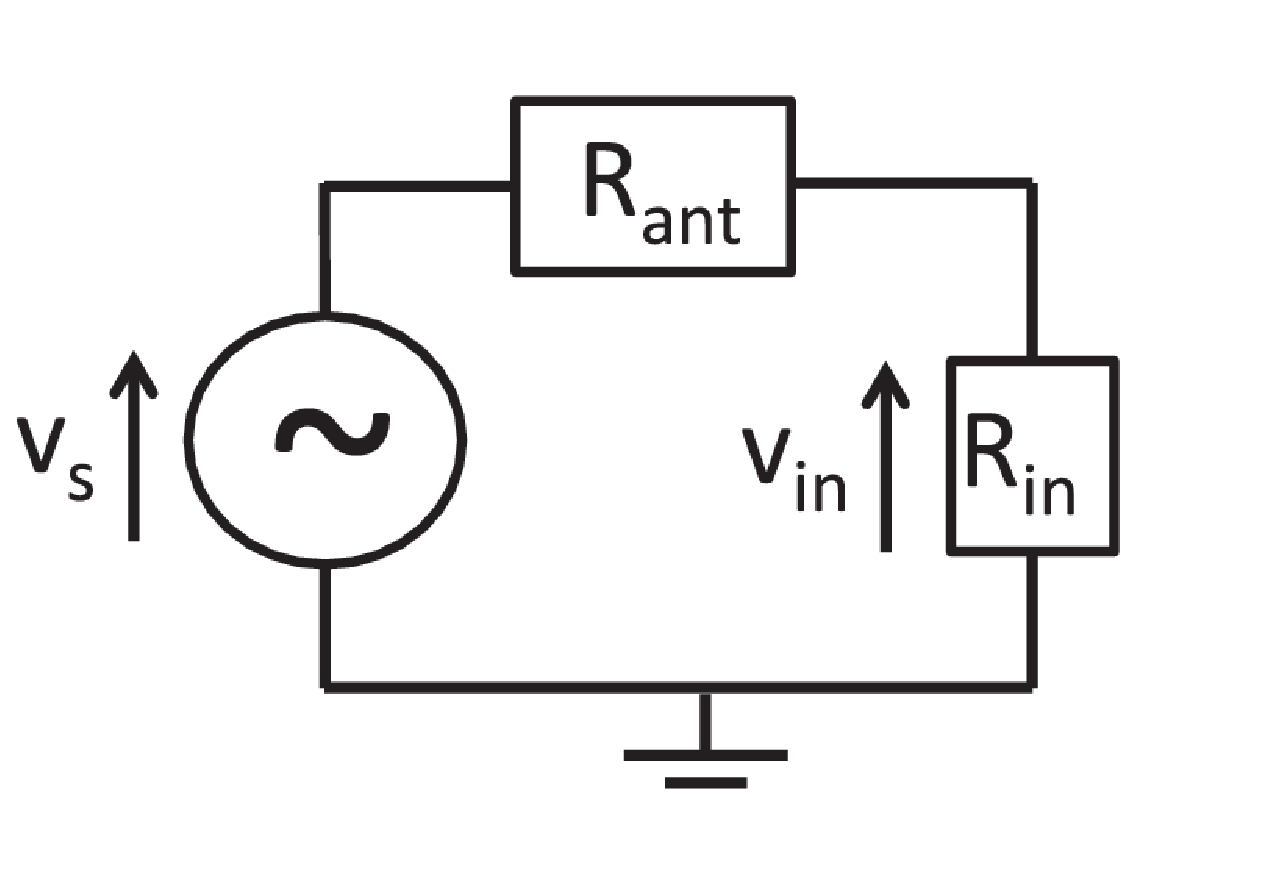
\includegraphics[width=\linewidth]{assets/antenna_equivalent_circuit.eps}
				\caption{Antenna equivalent circuit}
				\label{fi:antenna_equivalent_circuit}
			\end{subfigure}%
			~
			\begin{subfigure}[t]{0.45\linewidth}
				\centering
				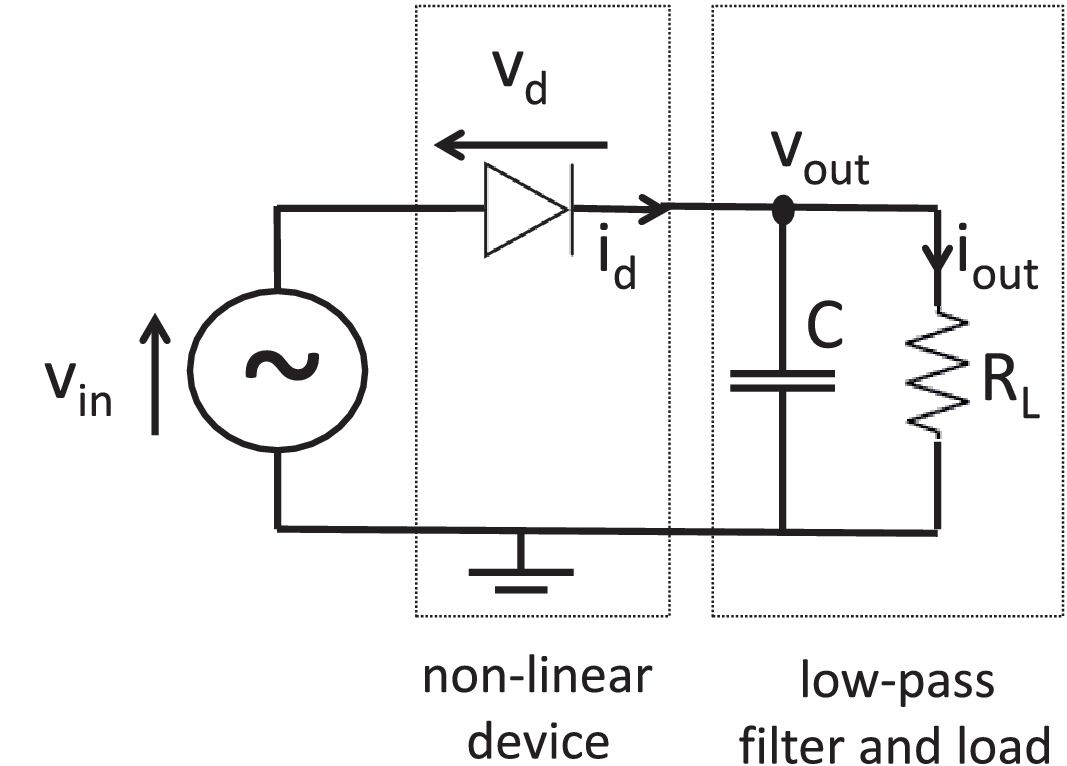
\includegraphics[width=\linewidth]{assets/single_diode_rectifier.eps}
				\caption{A single diode rectifier}
				\label{fi:single_diode_rectifier}
			\end{subfigure}
			\caption{Rectenna circuit}
		\end{figure}

		Rectifiers consist of nonlinear components as diode and capacitor to produce DC and store energy \cite{Hagerty2004,Pinuela2013}. Consider a simplified rectifier in Fig. \ref{fi:single_diode_rectifier} where a single series diode is followed by a low-pass filter with load. Denote $v_d(t)=v_{\text{in}}(t)-v_{\text{out}}(t)$ as the voltage across the diode where $v_{\text{out}}(t)$ is the output voltage across the load. A Taylor expansion of the diode characteristic equation $i_d(t)=i_s(e^{v_d(t)/n' v_t}-1)$ (with $i_s$ the reverse bias saturation current, $n'$ the diode ideality factor, $v_t$ the thermal voltage) around a quiescent operating point $v_d=a$ writes as $i_d(t)=\sum_{i=0}^{\infty}k_i'(v_d(t)-a)^i$, where $k_0'=i_s(e^{a/n' v_t}-1)$ and $k_i'=i_se^{a/n'v_t}/i!(n'v_t)^i,i=1,\dots,\infty$. Note that this small signal expansion model is only valid for the non-linear operation region, and the I-V relationship would be linear if the diode behavior is dominated by the load \cite{Clerckx2016a}. Also, an ideal low-pass filter with steady-state response can provide a constant $v_{\text{out}}$ that depends on the peak of $v_{\text{in}}(t)$ \cite{Curty2005}. Therefore, a proper choice of the operating voltage drop is $a=\mathcal{E}\{v_d(t)\}=-v_{\text{out}}$ such that
		\begin{equation}\label{eq:i_d}
			i_d(t)=\sum_{i=0}^{\infty}k_i'\rho^{i/2}R_{\text{ant}}^{i/2}y(t)^i
		\end{equation}

		By discarding non-DC components, taking expectation over symbol distribution, and truncating \ref{eq:i_d} to the $n_0$-th order, we approximate the average output DC current for a given channel as
		\begin{equation}\label{eq:i_out}
			i_{\text{out}}(t)=\mathcal{A}\{i_d(t)\}\approx\sum_{i=0}^{\infty}{k_i'}{\rho^{i/2}}{R_{\text{ant}}^{i/2}}\mathcal{E}\left\{{\mathcal{A}\left\{y(t)^i\right\}}\right\}
		\end{equation}

		With the assumption of evenly spaced frequencies, it holds that $\mathcal{A}\left\{y(t)^i\right\}=0$ for odd $i$ thus the related terms has no contribution to DC components. However, $k_i'$ is still a function of $i_{\text{out}}$, and \cite{Clerckx2016a} proved that maximizing a truncated $i_{\text{out}}$ is equivalent to maximizing a monotonic function
		\begin{equation}\label{eq:z}
			z(\boldsymbol{\phi},\boldsymbol{w}_I,\boldsymbol{w}_P,\rho)=\sum_{i\,\text{even},i\ge2}^{n_0}{k_i}{\rho^{i/2}}{R_{\text{ant}}^{i/2}}{\mathcal{E}\left\{\mathcal{A}\left\{y(t)^i\right\}\right\}}
		\end{equation}
		where $k_i=i_s/i!(nv_t)^i$. It can be observed that the traditional linear harvester model, where the output DC power equals the sum of the power harvested on each frequency, is a special case of \ref{eq:z} with $n_0=2$. However, due to the coupling among different frequencies, some high-order terms also cancel out non-DC components thus contribute to the output DC power. In other words, even terms with $i \ge 4$ account for the nonlinear behavior of the diode. For simplicity, we choose $n_0=4$ to investigate fundamental nonlinearity and let $\beta_2={k_2}{R_{\text{ant}}}$, $\beta_4={k_4}{R_{\text{ant}}^2}$. Note that $\mathcal{E}\left\{\lvert\tilde{x}_{I,n}\rvert^2\right\}=1$ but $\mathcal{E}\left\{\lvert\tilde{x}_{I,n}\rvert^4\right\}=2$ can be interpreted as a modulation gain on the nonlinear terms of the output DC current.

		Similar to \cite{Huang2017}, we further stack up channel and waveform vectors over all subbands to define $\boldsymbol{h}=[\boldsymbol{h}_1^H,\dots,\boldsymbol{h}_N^H]^H \in \mathbb{C}^{MN \times 1}$, $\boldsymbol{w}_{I/P}=[\boldsymbol{w}_{I/P,1}^H,\dots,\boldsymbol{w}_{I/P,N}^H]^H \in \mathbb{C}^{MN \times 1}$. Moreover, let $\boldsymbol{W}_{I/P,n}$ keep the $n$-th ($n=-N+1,\dots,N-1$) block diagonal of $\boldsymbol{W}_{I/P}=\boldsymbol{w}_{I/P}\boldsymbol{w}_{I/P}^H$ and null the remaining entries. On top of this, $z$ is reduced to \ref{eq:z_expand} with DC terms expressed in \ref{eq:y_I2} -- \ref{eq:y_P4}.
		\begin{figure*}[b]
			\hrule
			\begin{align}
				z(\boldsymbol{\phi},\boldsymbol{w}_I,\boldsymbol{w}_P,\rho)
				& = \beta_2\rho\Bigl(\mathcal{E}\left\{\mathcal{A}\left\{y_{I}^2(t)\right\}\right\}+\mathcal{A}\left\{y_{P}^2(t)\right\}\Bigr)+\beta_4\rho^2\Bigl(\mathcal{E}\left\{\mathcal{A}\left\{y_{I}^4(t)\right\}\right\}+\mathcal{A}\left\{y_{P}^4(t)\right\}+6\mathcal{E}\left\{\mathcal{A}\left\{y_{I}^2(t)\right\}\right\}\mathcal{A}\left\{y_{P}^2(t)\right\}\Bigr)\label{eq:z_expand}\\
				\mathcal{E}\left\{\mathcal{A}\left\{y_{I}^2(t)\right\}\right\}
				& = \frac{1}{2}\sum_{n=1}^N{(\boldsymbol{h}_{n}^H\boldsymbol{w}_{I,n})(\boldsymbol{h}_{n}^H\boldsymbol{w}_{I,n})^H} = \frac{1}{2}\boldsymbol{h}^H\boldsymbol{W}_{I,0}\boldsymbol{h}\label{eq:y_I2}\\
				\mathcal{E}\left\{\mathcal{A}\left\{y_{I}^4(t)\right\}\right\}
				& = \frac{3}{4}\left(\sum_{n=1}^N{(\boldsymbol{h}_{n}^H\boldsymbol{w}_{I,n})(\boldsymbol{h}_{n}^H\boldsymbol{w}_{I,n})^H}\right)^2 = \frac{3}{4}(\boldsymbol{h}^H\boldsymbol{W}_{I,0}\boldsymbol{h})^2\\
				\mathcal{A}\left\{y_{P}^2(t)\right\}
				& = \frac{1}{2}\sum_{n=1}^N{(\boldsymbol{h}_{n}^H\boldsymbol{w}_{P,n})(\boldsymbol{h}_{n}^H\boldsymbol{w}_{P,n})^H} = \frac{1}{2}\boldsymbol{h}^H\boldsymbol{W}_{P,0}\boldsymbol{h}\\
				\mathcal{A}\left\{y_{P}^4(t)\right\}
				& = \frac{3}{8}\sum_{\substack{{n_1},{n_2},{n_3},{n_4}\\{n_1}+{n_2}={n_3}+{n_4}}}{(\boldsymbol{h}_{{n_1}}^H\boldsymbol{w}_{P,{n_1}})(\boldsymbol{h}_{{n_2}}^H\boldsymbol{w}_{P,{n_2}})(\boldsymbol{h}_{{n_3}}^H\boldsymbol{w}_{P,{n_3}})^H(\boldsymbol{h}_{{n_4}}^H\boldsymbol{w}_{P,{n_4}})^H} = \frac{3}{8}\sum_{n=-N+1}^{N-1}(\boldsymbol{h}^H\boldsymbol{W}_{P,n}\boldsymbol{h})(\boldsymbol{h}^H\boldsymbol{W}_{P,n}\boldsymbol{h})^H\label{eq:y_P4}
			\end{align}
		\end{figure*}
	\end{subsection}

	\begin{subsection}{Rate-Energy Region}
		Define the achievable R-E region as
		\begin{equation}
			\begin{split}
				C_{R_{\text{ID}}-I_{\text{EH}}}(P)
				&\triangleq \biggl\{(R_{\text{ID}}, I_{\text{EH}}): R_{\text{ID}} \le R, I_{\text{EH}} \le z,\\
				&\quad \frac{1}{2}\left(\lVert{\boldsymbol{w}_I}\rVert^2+\lVert{\boldsymbol{w}_P}\rVert^2\right) \le P\biggr\}
			\end{split}
		\end{equation}
		where $P$ is the average transmit power budget and the coefficient $1/2$ converts the maximum power of sine waves to the average power.
	\end{subsection}
\end{section}

\begin{section}{Problem Formulation}
	We characterize the R-E region through multiple current maximization problems subject to transmit power, IRS magnitude, and different rate constraints
	\begin{maxi!}
		{\boldsymbol{\phi},\boldsymbol{w}_I,\boldsymbol{w}_P,\rho}{z(\boldsymbol{\phi},\boldsymbol{w}_I,\boldsymbol{w}_P,\rho)}{\label{op:original}}{\label{ob:original}}
		\addConstraint{\frac{1}{2}\left(\lVert{\boldsymbol{w}_I}\rVert^2+\lVert{\boldsymbol{w}_P}\rVert^2\right)\le{P}}\label{co:original_power}
		\addConstraint{R(\boldsymbol{\phi},\boldsymbol{w}_I,\rho) \ge \bar{R}}\label{co:original_rate}
		\addConstraint{\lvert{\phi_l}\rvert=1, \quad l=1,\dots,L}\label{co:original_modulus}
		\addConstraint{0 \le \rho \le 1}
	\end{maxi!}
	Problem \ref{op:original} is intricate with coupled variables involved in non-convex objective function \ref{ob:original} and rate constraint \ref{co:original_rate}. To reduce the design complexity, we propose an suboptimal AO algorithm that iteratively updates the IRS phase shift and transmit waveform together with receive splitting ratio until convergence.

	\begin{subsection}{IRS Phase Shift}
		In this section, the IRS phase shift $\boldsymbol{\phi}$ is optimized for any given waveform $\boldsymbol{w}_{I/P}$ and splitting ratio $\rho$. We observe that
		\begin{equation}
			\begin{split}
				\lvert \boldsymbol{h}_{n}^H\boldsymbol{w}_{I,n} \rvert^2
				& = \boldsymbol{w}_{I,n}^H\boldsymbol{h}_n\boldsymbol{h}_n^H\boldsymbol{w}_{I,n}\\
				& = \boldsymbol{w}_{I,n}^H(\boldsymbol{h}_{D,n}+\boldsymbol{V}_n^H\boldsymbol{\phi})(\boldsymbol{h}_{D,n}^H+\boldsymbol{\phi}^H\boldsymbol{V}_n)\boldsymbol{w}_{I,n}\\
				& = \boldsymbol{w}_{I,n}^H\boldsymbol{M}_n^H\boldsymbol{\Phi}\boldsymbol{M}_n\boldsymbol{w}_{I,n}\\
				& = \mathrm{Tr}(\boldsymbol{M}_n\boldsymbol{w}_{I,n}\boldsymbol{w}_{I,n}^H\boldsymbol{M}_n^H\boldsymbol{\Phi})\\
				& = \mathrm{Tr}(\boldsymbol{C}_n\boldsymbol{\Phi})
			\end{split}
		\end{equation}
		where $t$ is an auxiliary variable with unit modulus, $\boldsymbol{M}_n=[\boldsymbol{V}_n^H, \boldsymbol{h}_{D,n}]^H \in \mathbb{C}^{(L+1) \times M}$, $\bar{\boldsymbol{\phi}}=[\boldsymbol{\phi}^H, t]^H \in \mathbb{C}^{(L+1) \times 1}$, $\boldsymbol{\Phi}=\bar{\boldsymbol{\phi}}\bar{\boldsymbol{\phi}}^H \in \mathbb{C}^{(L+1) \times (L+1)}$, $\boldsymbol{C}_n = \boldsymbol{M}_n\boldsymbol{w}_{I,n}\boldsymbol{w}_{I,n}^H\boldsymbol{M}_n^H \in \mathbb{C}^{(L+1)\times(L+1)}$. Similarly, we define $t_{I/P,n}$ ($n=-N+1,\dots,N-1$) as
		\begin{equation}
			\begin{split}
				t_{I/P,n}
				& = \boldsymbol{h}^H\boldsymbol{W}_{I/P,n}\boldsymbol{h}\\
				& = \mathrm{Tr}(\boldsymbol{h}\boldsymbol{h}^H\boldsymbol{W}_{I/P,n})\\
				& = \mathrm{Tr}\left((\boldsymbol{h}_{D}+\boldsymbol{V}^H\boldsymbol{\phi})(\boldsymbol{h}_{D}^H+\boldsymbol{\phi}^H\boldsymbol{V})\boldsymbol{W}_{I/P,n}\right)\\
				& = \mathrm{Tr}(\boldsymbol{M}^H\boldsymbol{\Phi}\boldsymbol{M}\boldsymbol{W}_{I/P,n})\\
				& = \mathrm{Tr}(\boldsymbol{M}\boldsymbol{W}_{I/P,n}\boldsymbol{M}^H\boldsymbol{\Phi})\\
				& = \mathrm{Tr}(\boldsymbol{C}_{I/P,n}\boldsymbol{\Phi})
			\end{split}
		\end{equation}
		where $\boldsymbol{h}_D=[\boldsymbol{h}_{D,1}^H,\dots,\boldsymbol{h}_{D,N}^H]^H \in \mathbb{C}^{MN \times 1}$, $\boldsymbol{V}=[\boldsymbol{V}_1,\dots,\boldsymbol{V}_N] \in \mathbb{C}^{L \times MN}$, $\boldsymbol{M}=[\boldsymbol{V}^H, \boldsymbol{h}_{D}]^H \in \mathbb{C}^{(L+1) \times MN}$, $\boldsymbol{C}_{I/P,n}=\boldsymbol{M}\boldsymbol{W}_{I/P,n}\boldsymbol{M}^H \in \mathbb{C}^{(L+1)\times(L+1)}$. Therefore, the rate and objective expressions \ref{eq:R} and \ref{eq:z_expand} rewrites as \ref{eq:R_irs} and \ref{eq:z_irs}, respectively.
		\begin{equation}\label{eq:R_irs}
			R(\boldsymbol{\Phi}) = \sum_{n}{\log_2\left(1+\frac{(1-\rho)\mathrm{Tr}(\boldsymbol{C}_n\boldsymbol{\Phi})}{\sigma_n^2}\right)}
		\end{equation}
		\begin{equation}\label{eq:z_irs}
			\begin{split}
				z(\boldsymbol{\Phi})
				&=\frac{1}{2}{\beta_2}{\rho}(t_{I,0}+t_{P,0})\\
				&\quad+\frac{3}{8}{\beta_4}{\rho^2} \left(2t_{I,0}^2 + \sum_{n=-N+1}^{N-1}{t_{P,n}t_{P,n}^*}\right)\\
				&\quad+\frac{3}{2}{\beta_4}{\rho^2}t_{I,0}t_{P,0}
			\end{split}
		\end{equation}

		To maximize non-concave expression \ref{eq:z_irs}, we propose a Successive Convex Approximation (SCA)-based algorithm that approximate the second-order terms by first-order Taylor expansion. Based on the variables optimized at iteration $i - 1$, the local approximation at iteration $i$ suggests \cite{Adali2010}
		\begin{align}
			(t_{I,0}^{(i)})^2
			& \ge 2 t_{I,0}^{(i)}t_{I,0}^{(i-1)} - (t_{I,0}^{(i-1)})^2\label{eq:taylor_1}\\
			t_{P,n}^{(i)} (t_{P,n}^{(i)})^*
			& \ge 2 \Re\left\{t_{P,n}^{(i)} (t_{P,n}^{(i-1)})^*\right\} - t_{P,n}^{(i-1)} (t_{P,n}^{(i-1)})^*\label{eq:taylor_2}\\
			t_{I,0}^{(i)} t_{P,0}^{(i)}
			& = \frac{1}{4}(t_{I,0}^{(i)} + t_{P,0}^{(i)})^2 - \frac{1}{4}(t_{I,0}^{(i)} - t_{P,0}^{(i)})^2\nonumber\\
			& \ge \frac{1}{2}(t_{I,0}^{(i)} + t_{P,0}^{(i)})(t_{I,0}^{(i-1)} + t_{P,0}^{(i-1)})\nonumber\\
			& \quad - \frac{1}{4}(t_{I,0}^{(i-1)} + t_{P,0}^{(i-1)})^2 - \frac{1}{4}(t_{I,0}^{(i)} - t_{P,0}^{(i)})^2\label{eq:taylor_3}
		\end{align}
		which provide lower bounds to the corresponding terms in \ref{eq:z_irs}. At iteration $i$, the approximated objection function $\tilde{z}(\boldsymbol{\Phi}^{(i)})$ is detailed in \ref{eq:z_irs_approx}.
		\begin{figure*}[b]
			\hrule
			\begin{equation}\label{eq:z_irs_approx}
				\begin{split}
					\tilde{z}(\boldsymbol{\Phi}^{(i)})
					& = \frac{1}{2}{\beta_2}{\rho}(t_{I,0}^{(i)}+t_{P,0}^{(i)})\\
					& \quad + \frac{3}{8}{\beta_4}{\rho^2} \left(4 (t_{I,0}^{(i)})(t_{I,0}^{(i-1)}) - 2 (t_{I,0}^{(i-1)})^2 + \sum_{n=-N+1}^{N-1}{2 \Re\left\{t_{P,n}^{(i)} (t_{P,n}^{(i-1)})^*\right\} - t_{P,n}^{(i-1)} (t_{P,n}^{(i-1)})^*}\right)\\
					& \quad + \frac{3}{2}{\beta_4}{\rho^2} \left(\frac{1}{2}(t_{I,0}^{(i)} + t_{P,0}^{(i)})(t_{I,0}^{(i-1)} + t_{P,0}^{(i-1)}) - \frac{1}{4}(t_{I,0}^{(i-1)} + t_{P,0}^{(i-1)})^2 - \frac{1}{4}(t_{I,0}^{(i)} - t_{P,0}^{(i)})^2\right)
				\end{split}
			\end{equation}
		\end{figure*}
		Hence, problem \ref{op:original} is transformed to
		\begin{maxi!}
			{\boldsymbol{\boldsymbol{\Phi}}}{\tilde{z}(\boldsymbol{\Phi})}{\label{op:irs}}{\label{ob:irs}}
			\addConstraint{R(\boldsymbol{\Phi}) \ge \bar{R}}\label{co:irs_rate}
			\addConstraint{\boldsymbol{\Phi}_{l,l}=1, \quad l=1,\dots,L+1}\label{co:irs_modulus}
			\addConstraint{\boldsymbol{\Phi}\succeq{0}}
			\addConstraint{\mathrm{rank}(\boldsymbol{\Phi})=1\label{co:irs_rank}}
		\end{maxi!}

		Problem \ref{op:irs} is not a standard Semidefinite Programming (SDP) due to the rate constraint \ref{co:irs_rate}. Therefore, even if we relax the rank constraint \ref{co:irs_rank} to formulate a convex problem, there is no guarantee that the optimal rank-1 solution $\bar{\boldsymbol{\phi}}^{\star}$ extracted from $\boldsymbol{\Phi}^{\star}$ is a stationary point of the original problem \ref{op:original}. In Section [TODO], we numerically show that $\boldsymbol{\Phi}^{\star}$ is rank-1 for all tested channel realizations so that the performance loss is insignificant.

		When $\boldsymbol{\Phi}^{\star}$ is rank-1, the optimal phase shift vector $\bar{\boldsymbol{\phi}}^\star$ is obtained by Eigenvalue Decomposition (EVD). Otherwise, a suboptimal solution can be extracted via Gaussian randomization method \cite{Huang2010}. Specifically, we perform EVD $\boldsymbol{\Phi}^{\star}=\boldsymbol{U}\boldsymbol{\Sigma}\boldsymbol{U}^H$, generate $Q$ CSCG random vectors $\boldsymbol{r}_q \sim \mathcal{CN}(\boldsymbol{0},\boldsymbol{I}_{L+1}),\ q=1,\dots,Q$, construct the corresponding candidates $\bar{\boldsymbol{\phi}}_q=e^{j\arg\left(\boldsymbol{U}\boldsymbol{\Sigma}^{1/2}\boldsymbol{r}_q\right)}$, and choose the one that maximizes the objective function \ref{ob:irs}. Finally, the phase shift is retrieved by $\theta_l=\arg(\phi_l^\star/\phi_{L+1}^\star), \ l=1,\dots,L$. The algorithm for the phase shift optimization is summarized in Algorithm \ref{al:irs}.
		\begin{algorithm}
			\caption{SCA: IRS Phase Shift}
			\label{al:irs}
			\begin{algorithmic}[1]
				\State \textbf{Input} $\beta_2,\beta_4,\boldsymbol{h}_D,\boldsymbol{h}_I,\boldsymbol{h}_R,\boldsymbol{w}_I,\boldsymbol{w}_P,\rho,\sigma_n,\bar{R},Q,\epsilon$
				\State Construct $\boldsymbol{M},\boldsymbol{M}_n,\boldsymbol{C}_{n}$ for $n=1,\dots,N$, $\boldsymbol{C}_{I/P,n}$ for $n=-N+1,\dots,N-1$
				\State \textbf{Initialize} $i \gets 0,\boldsymbol{\Phi}^{(0)},t_{I/P,n}^{(0)}$, $n=-N+1,\dots,N-1$
				\Repeat
					\State $i \gets i + 1$
					\State Obtain $\boldsymbol{\Phi}^{(i)}, t_{I/P,n}^{(i)}$ by solving problem \ref{op:irs}
					\State Compute $z^{(i)}$ by \ref{eq:z_irs}
				\Until $\lvert (z^{(i)}-z^{(i-1)}) / z^{(i)} \rvert \le \epsilon$
				\State Set $\boldsymbol{\Phi}^{\star}=\boldsymbol{\Phi}^{(i)}$
				\If{$\mathrm{rank}(\boldsymbol{\Phi}^{\star})=1$}
					\State Obtain $\bar{\boldsymbol{\phi}}^\star$ by $\boldsymbol{\Phi}^{\star}=\bar{\boldsymbol{\phi}}^\star(\bar{\boldsymbol{\phi}}^\star)^H$
				\Else
					\State Obtain $\boldsymbol{U},\boldsymbol{\Sigma}$ by $\boldsymbol{\Phi}^{\star}=\boldsymbol{U}\boldsymbol{\Sigma}\boldsymbol{U}^H$

					\State Generate $\boldsymbol{r}_q \sim \mathcal{CN}(\boldsymbol{0},\boldsymbol{I}_{L+1})$, $q=1,\dots,Q$
					\State Construct $\bar{\boldsymbol{\phi}}_q=e^{j\arg\left(\boldsymbol{U}\boldsymbol{\Sigma}^{1/2}\boldsymbol{r}_q\right)}$, $\boldsymbol{\Phi}_q=\bar{\boldsymbol{\phi}}_q\bar{\boldsymbol{\phi}}_q^H$
					\State Set $q^{\star}=\arg\max_q{z(\boldsymbol{\Phi}_q)}$, $\bar{\boldsymbol{\phi}}^\star=\bar{\boldsymbol{\phi}}_{q^{\star}}$
				\EndIf
				\State Set $\theta_l^\star=\arg(\phi_l^\star/\phi_{L+1}^\star), \ l=1,\dots,L$
				\State \textbf{Output} $\boldsymbol{\phi}^{\star}$
			\end{algorithmic}
		\end{algorithm}
	\end{subsection}

	\begin{subsection}{Waveform and Splitting Ratio}
		Next, we jointly optimize both information and power waveforms $\boldsymbol{w}_{I/P}$ together with splitting ratio $\rho$ for any given IRS phase shift $\boldsymbol{\phi}$. As pointed out in \cite{Clerckx2018b}, the waveform design in frequency and spatial domain can be decoupled without performance loss, and the optimal spatial weight is given by Maximum-Ratio Transmission (MRT) beamformer
		\begin{equation}\label{eq:w_IP}
			\boldsymbol{w}_{I/P,n}=s_{I/P,n}\frac{\boldsymbol{h}_n}{\lVert{\boldsymbol{h}_n}\rVert}
		\end{equation}
		That is to say, it is only necessary to determine the amplitudes $s_{I/P,n}$ at different tones for single-user MISO SWIPT, and the original waveform optimization with $2MN$ variables is converted into a power allocation problem with $2N$ nonnegative real variables. Let $\boldsymbol{s}_{I/P}=[s_{I/P,1},\dots,s_{I/P,N}]^T \in \mathbb{C}^{N \times 1}$. At subband $n$, the effective channel gain is given by $\lVert{\boldsymbol{h}_n}\rVert$ and the power allocated to the modulated and unmodulated waveform are given by $s_{I,n}^2$ and $s_{P,n}^2$, respectively. With such a beamformer selection, we have $\boldsymbol{h}_n^H\boldsymbol{w}_{I,n}=\lvert{\boldsymbol{h}_n^H\boldsymbol{w}_{I,n}}\rvert=\lVert{\boldsymbol{h}_n}\rVert s_{I,n}$ such that the rate and objective expressions \ref{eq:R} and \ref{eq:z_expand} reduces to \ref{eq:R_waveform} and \ref{eq:z_waveform}.
		\begin{equation}\label{eq:R_waveform}
			R(\boldsymbol{s}_I,\rho) = \log_2\left(\prod_{n=1}^N\biggl(1+\frac{(1-\rho)\lVert{\boldsymbol{h}_n}\rVert^2 s_{I,n}^2}{\sigma_n^2}\biggr)\right)
		\end{equation}
		\begin{figure*}[b]
			\hrule
			\begin{equation}\label{eq:z_waveform}
				\begin{split}
					z(\boldsymbol{s}_I,\boldsymbol{s}_P,\rho)
					& = \frac{1}{2}{\beta_2}{\rho} \sum_{n=1}^N \lVert{\boldsymbol{h}_n}\rVert^2(s_{I,n}^2+s_{P,n}^2)\\
					& \quad + \frac{3}{8}{\beta_4}{\rho^2} \left( 2\sum_{n_1,n_2} \prod_{j=1}^2 \lVert{\boldsymbol{h}_{n_j}}\rVert^2 s_{I,{n_j}}^2 + \sum_{\substack{{n_1},{n_2},{n_3},{n_4}\\{n_1}+{n_2}={n_3}+{n_4}}} \prod_{j=1}^4 \lVert{\boldsymbol{h}_{n_j}}\rVert s_{I,{n_j}} \right)\\
					& \quad + \frac{3}{2}{\beta_4}{\rho^2} \left( \sum_{n_1,n_2} \lVert{\boldsymbol{h}_{n_1}}\rVert^2 s_{I,{n_1}}^2 \lVert{\boldsymbol{h}_{n_2}}\rVert^2 s_{P,{n_2}}^2 \right)
				\end{split}
			\end{equation}
		\end{figure*}
		Therefore, \ref{op:original} is reduced to an amplitude optimization problem
		\begin{maxi!}
			{\boldsymbol{s}_I,\boldsymbol{s}_P,\rho}{z(\boldsymbol{s}_I,\boldsymbol{s}_P,\rho)}{\label{op:waveform}}{}
			\addConstraint{\frac{1}{2}\left(\lVert{\boldsymbol{s}_I}\rVert^2+\lVert{\boldsymbol{s}_P}\rVert^2\right)\le{P}}
			\addConstraint{R(\boldsymbol{s}_I,\rho) \ge \bar{R}}
		\end{maxi!}
		Since problem \ref{op:waveform} involves the production of nonnegative real variables, we introduce auxiliary variables $t',\bar{\rho}$ and transform it into a reversed GP
		\begin{mini!}
			{\boldsymbol{s}_I,\boldsymbol{s}_P,\rho,\bar{\rho},t'}{\frac{1}{t'}}{\label{op:waveform_rgp}}{}
			\addConstraint{\frac{1}{2}\left(\lVert{\boldsymbol{s}_I}\rVert^2+\lVert{\boldsymbol{s}_P}\rVert^2\right) \le P}\label{co:waveform_power}
			\addConstraint{\frac{t'}{z(\boldsymbol{s}_I,\boldsymbol{s}_P,\rho)} \le 1}\label{co:waveform_objective}
			\addConstraint{\frac{2^{\bar{R}}}{\prod_{n=1}^N \left(1+{\bar{\rho}\lVert{\boldsymbol{h}_n}\rVert^2 s_{I,n}^2}/{\sigma_n^2}\right)} \le 1}\label{co:waveform_rate}
			\addConstraint{\rho + \bar{\rho} \le 1}
		\end{mini!}
		It is observed that the denominators of \ref{co:waveform_objective}, \ref{co:waveform_rate} are posynomials \cite{Boyd2007}, and we further express them in a compact form
		\begin{align}
			z(\boldsymbol{s}_I,\boldsymbol{s}_P,\rho)&=\sum_{m_P}{g_{m_P}(\boldsymbol{s}_I,\boldsymbol{s}_P,\rho)}\label{eq:posynomial_objective}\\
			1+\frac{\bar{\rho}\lVert{\boldsymbol{h}_n}\rVert^2 s_{I,n}^2}{\sigma_n^2}&=\sum_{m_{I,n}}g_{m_{I,n}}(s_{I,n},\bar{\rho})\label{eq:posynomial_rate}
		\end{align}
		where $m_P,m_{I,n}$ are the number of monomials in the corresponding posynomials (obviously $m_{I,n}=2$). It is suggested in \cite{Clerckx2018b,Chiang2005} that posynomials \ref{eq:posynomial_objective} and \ref{eq:posynomial_rate} can be upper bounded by Arithmetic Mean-Geometric Mean (AM-GM) inequality such that problem \ref{op:waveform_rgp} is equivalent to
		\begin{mini}
			{\boldsymbol{s}_I,\boldsymbol{s}_P,\rho,\bar{\rho},t'}{\frac{1}{t'}}{\label{op:waveform_gp}}{}
			\addConstraint{\frac{1}{2}\left(\lVert{\boldsymbol{s}_I}\rVert^2+\lVert{\boldsymbol{s}_P}\rVert^2\right)\le{P}}
			\addConstraint{{t'}\prod_{m_P}{\left(\frac{g_{{m_P}}(\boldsymbol{s}_I,\boldsymbol{s}_P,\rho)}{\gamma_{{m_P}}}\right)^{-\gamma_{{m_P}}}}\le{1}}
			\addConstraint{2^{\bar{R}}\prod_{n}\prod_{m_{I,n}}\left(\frac{g_{m_{I,n}}(s_{I,n},\bar{\rho})}{\gamma_{m_{I,n}}}\right)^{-\gamma_{m_{I,n}}}\le{1}}
			\addConstraint{\rho + \bar{\rho} \le 1}
		\end{mini}
		where $\gamma_{m_P},\gamma_{m_{I,n}} \ge 0$, $\sum_{m_P}\gamma_{m_P}=\sum_{m_{I,n}}\gamma_{m_{I,n}}=1$. The tightness of the AM-GM inequality depends on $\{\gamma_{m_P},\gamma_{m_{I,n}}\}$ that require successive update, and a feasible choice at iteration $i$ is \cite{Clerckx2018b}
		\begin{align}
			\gamma_{m_P}^{(i)} & = \frac{g_{m_P}(\boldsymbol{s}_I^{(i-1)},\boldsymbol{s}_P^{(i-1)},\rho^{(i-1)})}{z(\boldsymbol{s}_I^{(i-1)},\boldsymbol{s}_P^{(i-1)},\rho^{(i-1)})}\label{eq:gamma_P}\\
			\gamma_{m_{I,n}}^{(i)} & = \frac{g_{m_{I,n}}(s_{I,n}^{(i-1)},\bar{\rho}^{(i-1)})}{1+{\bar{\rho}^{(i-1)}\lVert{\boldsymbol{h}_n}\rVert^2 (s_{I,n}^{(i-1)})^2}/{\sigma_n^2}}\label{eq:gamma_I}
		\end{align}
		$\boldsymbol{s}_I,\boldsymbol{s}_P,\rho$ are updated iteratively until convergence and the GP algorithm is summarized in Algorithm \ref{al:waveform}. It is also known as a inner approximation algorithm that only provides a KKT solution \cite{Marks1978}.
		\begin{algorithm}
			\caption{GP: Waveform and Splitting Ratio}
			\label{al:waveform}
			\begin{algorithmic}[1]
				\State \textbf{Input} $\beta_2,\beta_4,\boldsymbol{h},P,\sigma_n,\bar{R},\epsilon$
				\State \textbf{Initialize} $i \gets 0$, $\boldsymbol{s}_{I/P}^{(0)}$, $\rho^{(0)}$
				\Repeat
					\State $i \gets i + 1$
					\State Update $\{\gamma_{m_P}^{(i)},\gamma_{m_{I,n}}^{(i)}\}$ by \ref{eq:gamma_P}, \ref{eq:gamma_I}
					\State Obtain $\boldsymbol{s}_{I/P}^{(i)},\rho^{(i)}$ by solving problem \ref{op:waveform_gp}
					\State Compute $z^{(i)}$ by \ref{eq:z_waveform}
				\Until $\lvert (z^{(i)} - z^{(i-1)}) / z^{(i)} \rvert \le \epsilon$
				\State Set $\boldsymbol{s}_{I/P}^{\star}=\boldsymbol{s}_{I/P}^{(i)}$, $\rho^{\star}=\rho^{(i)}$, retrieve $\boldsymbol{w}_{I/P}^{\star}$ by \ref{eq:w_IP}
				\State \textbf{Output} $\boldsymbol{w}_{I/P}^{\star}, \rho^{\star}$
			\end{algorithmic}
		\end{algorithm}
	\end{subsection}

	\begin{subsection}{Alternating Optimization}
		For any direct, incident and reflective channels, we iteratively update the IRS phase shift by Algorithm \ref{al:irs} and transmit waveform together with receive splitting ratio by Algorithm \ref{al:waveform} until convergence. The alternating algorithm is summarized in Algorithm \ref{al:alternating}.
		\begin{algorithm}
			\caption{Alternating Algorithm for Problem \ref{op:original}}
			\label{al:alternating}
			\begin{algorithmic}[1]
				\State \textbf{Input} $\beta_2,\beta_4,\boldsymbol{h}_D,\boldsymbol{h}_I,\boldsymbol{h}_R,P,\sigma_n,\bar{R},Q,\epsilon$
				\State \textbf{Initialize} $i \gets 0$, $\boldsymbol{\phi}^{(0)},\boldsymbol{w}_{I/P}^{(0)},\rho^{(0)}$
				\Repeat
					\State $i \gets i + 1$
					\State Fix $\boldsymbol{w}_{I/P}^{(i-1)},\rho^{(i-1)}$ and obtain $\boldsymbol{\phi}^{(i)}$ by Algorithm \ref{al:irs}
					\State Fix $\boldsymbol{\phi}^{(i)}$, update $\boldsymbol{h}_n^{(i)}$, $n=1,\dots,N$ by \ref{eq:h_n} and obtain $\boldsymbol{w}_{I/P}^{(i)}, \rho^{(i)}$ by Algorithm \ref{al:waveform}
					\State Compute $z^{(i)}$ by \ref{eq:z_irs}
				\Until $\lvert (z^{(i)} - z^{(i-1)}) / z^{(i)} \rvert \le \epsilon$
				\State \textbf{Output} $\boldsymbol{\phi}^{\star}, \boldsymbol{w}_{I/P}^{\star}, \rho^{\star}$
			\end{algorithmic}
		\end{algorithm}
	\end{subsection}

	\begin{subsection}{Convergence and Complexity}
		\begin{subsubsection}{Convergence}
			The proposed alternating algorithm iteratively employs SCA-based IRS phase shift Algorithm \ref{al:irs} and GP-based waveform and splitting ratio Algorithm \ref{al:waveform} until convergence.

			\textbf{Proposition 1}. \textit{For any feasible initial point, the proposed SCA-based Algorithm \ref{al:irs} is guaranteed to converge to a stationary point of the IRS phase shift subproblem.}

			\textit{Proof:} The objective function \ref{ob:irs} is non-decreasing over iterations because the solution of problem \ref{op:irs} at iteration $i-1$ is still a feasible point at iteration $i$. Moreover, the sequence $\{\tilde{z}(\boldsymbol{\Phi}^{(i)})\}_{i=1}^{\infty}$ is bounded above due to the unit-modulus constraint \ref{co:irs_modulus}. Thus, Algorithm \ref{al:irs} is guaranteed to converge. To prove $\boldsymbol{\Phi}^{(i)}$ converge to the set of stationary points of IRS subproblem, we notice that the SCA-based Algorithm \ref{al:irs} is indeed an inner approximation algorithm \cite{Marks1978}, since $\tilde{z}(\boldsymbol{\Phi}) \le z(\boldsymbol{\Phi})$, $\partial\tilde{z}(\boldsymbol{\Phi}^{(i)})/\partial\boldsymbol{\Phi}=\partial z(\boldsymbol{\Phi}^{(i)})/\partial\boldsymbol{\Phi}$, and the approximation \ref{eq:taylor_1} -- \ref{eq:taylor_3} are asymptotically tight as $i \to \infty$ \cite{Adali2010,Li2013}. Therefore, Algorithm \ref{al:irs} converges to a stationary point.

			\textbf{Proposition 2}. \textit{For any feasible initial point, the GP-based Algorithm \ref{al:waveform} is guaranteed to converge to a stationary point of the waveform and splitting ratio subproblem.}

			\textit{Proof:} See \cite{Clerckx2016a,Clerckx2018b}.

			\textbf{Proposition 3}. \textit{Every limit point $(\boldsymbol{\phi}^{\star},\boldsymbol{w}_I^{\star},\boldsymbol{w}_P^{\star},\rho^{\star})$ of the proposed alternating algorithm is a stationary point of the original problem \ref{op:original}.}

			\textit{Proof:} The objective function \ref{ob:original} is non-decreasing over iterations of Algorithm \ref{al:alternating}, which is also upper-bounded due to the unit-modulus constraint \ref{co:original_modulus} and the average transmit power constraint \ref{co:original_power}. Thus, Algorithm \ref{al:alternating} is guaranteed to converge, namely the sequence $\{\boldsymbol{\phi}^{(i)},\boldsymbol{w}_I^{(i)},\boldsymbol{w}_P^{(i)},\rho^{(i)}\}$ generated by optimizing $\boldsymbol{\phi}$ and $\boldsymbol{w}_I,\boldsymbol{w}_P,\rho$ alternatively has limit points. As demonstrated in \cite{Grippo2000,Hong2016,Li2013a}, the solution is a stationary point of problem \ref{op:original}.
		\end{subsubsection}
	\end{subsection}
\end{section}

\begin{section}{Performance Evaluations}
	To evaluate the performance of the proposed IRS-aided SWIPT system, we characterize and compare typical R-E regions under different setups through simulations. Consider a large open space WiFi-like environment at a center frequency of 5.18 \si{GHz} with bandwidth $B=1$ \si{MHz}. The power delay profile of the frequency-selective fading channels are obtained from IEEE TGn NLOS channel model E \cite{Erceg2004}. Taps are modelled as i.i.d. CSCG random variables with normalized total power, and we assume no spatial correlation across all channels. The path loss model is given by
	\begin{equation}
		L(d)=L_0\left(\frac{d}{d_0}\right)^{-\alpha}
	\end{equation}
	where $L_0$ is the path loss at a reference distance $d_0$, $d$ is the distance between transmitter and receiver, $\alpha$ is the path loss exponent. We set $d_0=1$ \si{\metre}, $L_0=-30$ \si{\decibel}, and let $\alpha_D=3.8$, $\alpha_I=2.2$, $\alpha_R=2.2$ be the path loss exponents of direct, incident and reflective links, respectively. Rectenna parameters are taken as $k_2=0.0034$, $k_4=0.3829$, $R_{\text{ant}}=50$ \si{\ohm}. The average transmit power is fixed to $P=4$ \si{\W} while the average noise power is $\sigma_n=-60$ \si{\dBm} at all subbands. Each transmit/receive antenna and IRS element is assumed to have a $0$ \si{\dBi} antenna gain. Also, we choose a tolerance $\epsilon=10^{-8}$ and set $Q=10^{3}$ for the Gaussian randomization method.
\end{section}

\bibliographystyle{IEEEtran}
\bibliography{library.bib}
\end{document}
